%%%%%%%%%%%%%%%%%%%%%%%%%%%%% Define Article %%%%%%%%%%%%%%%%%%%%%%%%%%%%%%%%%%
\documentclass[journal,transmag]{IEEEtran}
%%%%%%%%%%%%%%%%%%%%%%%%%%%%%%%%%%%%%%%%%%%%%%%%%%%%%%%%%%%%%%%%%%%%%%%%%%%%%%%

%%%%%%%%%%%%%%%%%%%%%%%%%%%%% Using Packages %%%%%%%%%%%%%%%%%%%%%%%%%%%%%%%%%%
\usepackage{geometry}
\usepackage{graphicx}
\usepackage{amssymb}
\usepackage{amsmath}
\usepackage{amsthm}
\usepackage{empheq}
\usepackage{mdframed}
\usepackage{booktabs}
\usepackage{lipsum}
\usepackage{graphicx}
\usepackage{color}
\usepackage{psfrag}
\usepackage{pgfplots}
\usepackage{bm}
\usepackage[spanish]{babel}
\usepackage[utf8]{inputenc}
\usepackage{float}
%%%%%%%%%%%%%%%%%%%%%%%%%%%%%%%%%%%%%%%%%%%%%%%%%%%%%%%%%%%%%%%%%%%%%%%%%%%%%%%

% Other Settings

%%%%%%%%%%%%%%%%%%%%%%%%%% Page Setting %%%%%%%%%%%%%%%%%%%%%%%%%%%%%%%%%%%%%%%
\geometry{a4paper}

%%%%%%%%%%%%%%%%%%%%%%%%%% Define some useful colors %%%%%%%%%%%%%%%%%%%%%%%%%%
\definecolor{ocre}{RGB}{243,102,25}
\definecolor{mygray}{RGB}{243,243,244}
\definecolor{deepGreen}{RGB}{26,111,0}
\definecolor{shallowGreen}{RGB}{235,255,255}
\definecolor{deepBlue}{RGB}{61,124,222}
\definecolor{shallowBlue}{RGB}{235,249,255}
%%%%%%%%%%%%%%%%%%%%%%%%%%%%%%%%%%%%%%%%%%%%%%%%%%%%%%%%%%%%%%%%%%%%%%%%%%%%%%%

%%%%%%%%%%%%%%%%%%%%%%%%%% Define an orangebox command %%%%%%%%%%%%%%%%%%%%%%%%
\newcommand\orangebox[1]{\fcolorbox{ocre}{mygray}{\hspace{1em}#1\hspace{1em}}}
%%%%%%%%%%%%%%%%%%%%%%%%%%%%%%%%%%%%%%%%%%%%%%%%%%%%%%%%%%%%%%%%%%%%%%%%%%%%%%%

%%%%%%%%%%%%%%%%%%%%%%%%%%%% English Environments %%%%%%%%%%%%%%%%%%%%%%%%%%%%%
\newtheoremstyle{mytheoremstyle}{3pt}{3pt}{\normalfont}{0cm}{\rmfamily\bfseries}{}{1em}{{\color{black}\thmname{#1}~\thmnumber{#2}}\thmnote{\,--\,#3}}
\newtheoremstyle{myproblemstyle}{3pt}{3pt}{\normalfont}{0cm}{\rmfamily\bfseries}{}{1em}{{\color{black}\thmname{#1}~\thmnumber{#2}}\thmnote{\,--\,#3}}
\theoremstyle{mytheoremstyle}
\newmdtheoremenv[linewidth=1pt,backgroundcolor=shallowGreen,linecolor=deepGreen,leftmargin=0pt,innerleftmargin=20pt,innerrightmargin=20pt,]{theorem}{Theorem}[section]
\theoremstyle{mytheoremstyle}
\newmdtheoremenv[linewidth=1pt,backgroundcolor=shallowBlue,linecolor=deepBlue,leftmargin=0pt,innerleftmargin=20pt,innerrightmargin=20pt,]{definition}{Definition}[section]
\theoremstyle{myproblemstyle}
\newmdtheoremenv[linecolor=black,leftmargin=0pt,innerleftmargin=10pt,innerrightmargin=10pt,]{problem}{Problem}[section]
%%%%%%%%%%%%%%%%%%%%%%%%%%%%%%%%%%%%%%%%%%%%%%%%%%%%%%%%%%%%%%%%%%%%%%%%%%%%%%%

%%%%%%%%%%%%%%%%%%%%%%%%%%%%%%% Plotting Settings %%%%%%%%%%%%%%%%%%%%%%%%%%%%%
\usepgfplotslibrary{colorbrewer}
\pgfplotsset{width=8cm,compat=1.9}
%%%%%%%%%%%%%%%%%%%%%%%%%%%%%%%%%%%%%%%%%%%%%%%%%%%%%%%%%%%%%%%%%%%%%%%%%%%%%%%
\hyphenation{op-tical net-works semi-conduc-tor}

\begin{document}

\title{Cálculo diferencial e integral, Análisis Numérico}
\author{José Danilo Bonilla Vides, 00019520}
\markboth{Cálculo diferencial e integral, Análisis Numérico}%
{Shell \MakeLowercase{\textit{et al.}}: Bare Demo of IEEEtran.cls for IEEE Transactions on Magnetics Journals}

\IEEEtitleabstractindextext{%
\begin{abstract}
The abstract goes here.
\end{abstract}


\begin{IEEEkeywords}
IEEE, IEEEtran, IEEE Transactions on Magnetics, journal, \LaTeX, magnetics, paper, template.
\end{IEEEkeywords}}

\maketitle

\IEEEdisplaynontitleabstractindextext

\IEEEpeerreviewmaketitle

\section{Introducción}
El cálculo de las matemáticas es una de las ciencias más importantes para el desarrollo humano. \\
Desde el principio de los tiempos han existido diferentes técnicas y métodos que han ayudado 
a la población humana a poder resolver problemas prácticos en dónde las matemáticas son una parte
fundamental del proceso de la solución. \\

Teóricamente pueden modelarse ciertas funciones para poder ser resueltas con el fin de un enfoque pedagógico y de aprendizaje
pero en el ámbito profesional y práctico de la vida real, muchas veces se presentan ciertas funciones 
que suponen un desafío y una complejidad que no se puede resolver con las soluciones algebraicas que son
las que devuelven un valor exacto y preciso de la función. \\

Es por eso que existen técnicas y métodos que son llamados "Métodos Numéricos" o también a veces llamado "Soluciones Numéricas" 
que permiten resolver problemas que involucran funciones que son demasiado complejas
o no tienen una solución exacta por cálculos elementales. \\

Los métodos numéricos, denominados así porque, usualmente, consisten
en realizar una sucesión más o menos larga de operaciones numéricas (normalmente mediante la ayuda de un
ordenador), al cabo de las cuales encontramos un valor numérico que, si bien no es la solución exacta del
problema, se le parece mucho, es decir, aproxima la solución buscada con una precisión razonablemente buena. \cite{apunteClase}
\\
En este reporte se abordarán 4 métodos numéricos pertenecientes a la rama del Cálculo diferencial e integral.
\\
Los cuatro métodos numéricos que se abordarán en este reporte son: 
\begin{itemize}
    \item \textbf{Método de Romberg}
    \item  \textbf{Método de Simpson}
    \item   \textbf{Cuadratura Gaussiana}
    \item   \textbf{Diferencia media}
\end{itemize}
Existen ciertas aplicaciones en las que se puedan utilizar estos métodos, pero en las que se enfocará este reporte serán las 4 siguientes:
\begin{itemize}
    \item \textbf{Enésima derivada en un punto particular}
    \item \textbf{Cálculo de áreas}
    \item \textbf{Cálculo de volúmenes}
    \item \textbf{Sólidos de revolución}
\end{itemize}

\section{Método de Romberg}
\subsection{Descripción}

La integración de Romberg es una técnica diseñada para obtener integrales numéricas
de funciones de manera eficiente. Se basa en aplicaciones sucesivas de la regla del trapecio. \cite{chapra_mtodos_2007}
\\
Werner Romberg (1909–2093) concibió este procedimiento para mejorar la precisión de la regla 
trapezoidal al eliminar términos sucesivos en la expansión asintótica en 1955. \cite{burden_numerical_2016}
\\

Este método requiere del uso de la regla del trapecio de aplicación múltiple, además de 2 estimaciones de la integral para obtener una tercera estimación más exacta. \\

Deducción: \cite{chapra_mtodos_2007} \\
Si partimos del hecho de que se requieren 2 estimaciones y se conoce que la estimación y el error correspondiente a la regla del trapecio de aplicación
múltiple se representa de manera general como:
\begin{equation}
    I = I(h) + E(h)
\end{equation}
Donde $I$ es la estimación de la integral, $h$ es el paso de integración, $I(h)$ es la estimación de la integral con el paso de integración $h$, y $E(h)$ es el error de truncamiento. \\

Entonces nuestras 2 estimaciones, usando tamaño de paso $h_1$ y $h_2$, se representan de manera general como:
\begin{equation}
    I(h_1)+ E(h_1) = I(h_2) + E(h_2)
\end{equation}

Además el error de la regla trapezoidal múltiple puede representarse en forma aproximada con la ecuación:

\begin{equation} 
    E \approxeq \frac{b-a}{12}h^2f'' 
\end{equation}

Vamos a suponer que $f''$ es constante para cada paso en $h$, así podemos determinar la razón entre los dos errores, de las dos estimaciones que necesitamos, lo cuál sería: 
\begin{equation}
    \frac{E(h_1)}{E(h_2)} \approxeq \frac{h_1}{h_2}
\end{equation}

Reagrupamos la ecuación 4 para poder sustituirla en la ecuación 2:
\begin{equation}
    E(h_1) \approxeq E(h_2)\frac{h_1}{h_2}^2
\end{equation}

Al sustituir nos queda:
\begin{equation}
    I(h_1)+  E(h_2) \frac{h_1}{h_2}^2  \approxeq I(h_2) + E(h_2)
\end{equation}

Despejando $E(h_2)$:
\begin{equation}
    E(h_2) \approxeq \frac{I(h_1)-I(h_2)}{1- (h_1/h_2)^2}
\end{equation}

A fin de obtener una mejor estimación de la integral, podemos sustituir en la ecuación 1:
\begin{equation}
    I \approxeq I(h_2)+\frac{1}{(h_1/h_2)^2-1}|I(h_2)-I(h_1)|
\end{equation}

Al demostrarse el error de esta estimación, da como resultado $O(h^4)$. Es un resultado mayor al del error de estimación al utilizar solo la regla del trapecio ($O(h^2)$).
Este resultado se ha logrado al utilizar 2 estimaciones $O(h^2)$. \\

Si utilizamos un caso donde el paso $h_2$ es dividido por la mitad de $h_1$, la ecuación se convierte en:
\begin{equation}
    I \approxeq I(h_2)+\frac{1}{2^2-1}|I(h_2)-I(h_1)|
\end{equation}

Al simplificar y agrupar términos de la ecuación, obtenemos:
\begin{equation}
    I \approxeq \frac{4}{3}I(h_2)-\frac{1}{3}I(h_1)
\end{equation}

Este procedimiento es un subconjunto de un método más general para combinar integrales y obtener mejores estimaciones. \\

Entonces podemos seguir reduciendo el paso $h$ sucesivamente para obtener mejores estimaciones, por ejemplo al dividir nuevamente por la 
mitad la ecuación anterior obtenemos una exactitud de $O(h^6)$, quedando la siguiente ecuación:
\begin{equation}
    I \approxeq \frac{16}{15}I_m-\frac{1}{15}I_l
\end{equation}

Así podemos ir dividiendo por la mitad el paso $h$ y la exactitud irá mejorando en cada iteración. \\

Existe una forma general para representar todo este proceso con una ecuación, y es atribuida a Romberg, la cuál se representa de la siguiente manera:
\begin{equation}
    I_{j,k} \approxeq \frac{4^{k-1}I_{j+1, k-1}-I_{j,k-1}}{4^{k-1}-1}
\end{equation}

También es llamado Algoritmo de Integración de Romberg. \\

Dónde:
\begin{itemize}
\item $I_{j+1, k-1}$ es la integral más exacta,
\item  $I_{j, k-1}$ es la menos exacta,
\item $I_{j,k}$ es la integral mejorada,
\item $k$ significa el nivel de la integración
\item  $j$ se usa para distinguir entre las dos estimación más y menos exacta.
\end{itemize}

Esta ecuación es de las más adecuadas para llevar su implemntación a la computadora.






\subsection{Demostraciones de convergencia}
    Al aplicar el método de Romberg, y utilizando el nivel 1 de integración es decir, en el momento que $k=1$,
    se obtiene una estimación de la integral de $f$ entre $a$ y $b$, de manera que el error de la estimación es $O(h^2)$.
    Es decir que al utilizar $k=1$, se está utilizando la regla del trapecio para estimar la integral. \\

    Como este método se basa en dividir por la mitad el paso h en cada iteración, y con la deducción hecha, al utilizar el nivel 2, es decir con $k=2$, y $j=1$,
    se obtiene la ecuación:
    \begin{equation}
        I_{1,2} \approxeq \frac{4}{3}I_{2, 1}-\frac{1}{3}I_{1,1}
    \end{equation}

    La cual tiene una convergencia de $O(h^4)$, y así al ir aumentando el nivel de la integración, se va aumentando la exactitud de la estimación en ($h^{2n}$).
    Es decir la convergencia será mucho mayor por cada aumento del nivel de integración. \\
\subsection{Análisis del error}
    El criterio de paro o terminación puede darse mediante una ecuación del error relativo porcentual, para detenerse cuándo se esté satisfecho con los resultados obtenidos.
    La ecuación con un método útil para calcular el error relativo porcentual es la siguiente:
    \begin{equation}
        |E_a| = |\frac{I_{1,k}-I_{1,k-1}}{I_{1,k}}|100\%
    \end{equation}


\subsection{Análisis de la eficiencia del método}
    Evidentemente al tener una convergencia que aumenta en factor de $h^{2n}$, el método de Romberg es muy eficiente. 
    Sobretodo al compararlo con otros métodos y obtener las cantidades de iteraciones necesarias para obtener un resultado que satisfaga
    el criterio de paro, podemos determinar la eficiencia del método.  \\

    A continuación se presenta el ejemplo 22.1 de la página 652, obtenido de \cite{chapra_mtodos_2007} \\
        
    Teniendo la función $f(x)=0.2 + 25x - 200x^2 + 675x^3 - 900x^4 +400x^5 $ y el intervalo $[0,0.8]$.
    Al evaluarse esa integral, por medio de aplicaciones simples y múltiples de la regla del trapecio, se obtuvieron los siguientes resultados:

    \begin{table}[h]
        \begin{center}
            \caption{Ejemplo Analisis de la eficiencia del método}
            \begin{tabular}{| c | c | c | c |}
                \hline
            Segmentos & h & 0.1728 & ${E_t\%}$ \\ \hline
            1 & 0.8 & 0.1728 & 89.5 \\
            2 & 0.4 & 1.0688 & 34.9 \\
            4 & 0.2 & 1.4848 & 9.5 \\ \hline
            \end{tabular}
            \label{tab:ejemplo}
        \end{center}
            \end{table}
 
        Se utiliza el metodo de Romberg, para obtener una estimación de la integral,
        recordamos que con el nivel 1, cuando $k=1$, se obtiene el mismo resultado que el de la regla de trapecio.
        Cuándo utilizamos el nivel 2 de integración, es decir cuando $k=2$, se obtiene la siguiente ecuación:
        \begin{equation}
            I_{1,2} \approxeq \frac{4}{3}I_{2, 1}-\frac{1}{3}I_{1,1}
        \end{equation}
        
        Obteniendo un resultado de $I_{1,2}$ = 1.367467. \\

        Al trabajar con la siguiente iteración se obtiene un resultado de $I_{1,3}$ = 1.640533 \\

        Al trabajar con la iteración de nivel 4, obtenemos exactamente el mismo resultado $I_{1,3}$, por lo que hemos llegado 
        a nuestra condición de paro. \\

        Hemos llegado a la condición de paro en tan solo 3 iteraciones
        con el método de Romberg, al compararlo con otros métodos cómo por ejemplo
        la regla de Simpson, se obtiene una eficiencia mucho mejor, ya que realizando el ejemplo
        por el método de Simpson, este se tardaría 256 segmentos en poder llegar al mismo resultado
        obtenido con Romberg. \\

        Incluso, al exigir un resultado exacto con 7 cifras significativas, Romberg solo tarda 15 evaluaciones en poder
        obtener el resultado exacto, demostrando que es muy eficiente y que possee una convergencia mucho más veloz
        que la regla del trapecio y la regla de Simpson.

\subsection{Ventajas y desventajas del método}
    \subsubsection{Ventajas}
    \begin{center}
    Ventajas del método de Romberg:
    \end{center}
    \begin{itemize}
        \item   Es un método con una convergencia mucho más rápida que los demás métodos, 
        por ejemplo al compararlo con el método de Simpson y la regla del trapecio
        \item   Su convergencia aumenta a factor de $h^{2n}$ por cada iteración, brindando resultados muy veloces
        \item   La adaptación a la computarización del método por medio de la 
        ecuación de la forma general presentada por Romberg es de una dificultad baja para el que lo implementa,
        sin importar el lenguaje y/o software utilizado.
        \item   El cálculo del error relativo como condición de paro es muy intuitivo, fácil y rápido
    \end{itemize}
    \subsection{Desventajas}
    \begin{center}
    Desventajas del método de Romberg:
    \end{center}
    \begin{itemize}
        \item   Depende de conocer 2 estimaciones de la integral que se está calculando
        \item   No se puede trabajar con él sin conocer la función de la integral que se está buscando evaluar
        \item   Si se desea trabajar a mano, requiere un arduo trabajo, ya que se necesita calcular 
        el nuevo resultado por la regla del trapecio al aumentar el nivel de integración, es decir se hace 
        un doble trabajo por cada nueva iteración realizada.
    \end{itemize}

\subsection{Seudo-código}
        Seudo-código del método de Romberg: \cite{in_mr} \\

        ENTRADA: Extremos a, b; entero n $>$ 0 \\
        SALIDA: un arreglo R (calcule R por renglones; solo los 2 últimos renglones
        se guardan en almacenamiento) \\
        PROCESO: \\
        \begin{itemize}
            \item   PASO 1; tomar el valor de $h=(b-a)$; \\
                        $R_{1,1} = \frac{h}{2} (f(a)+f(b))$; \\
            \item   PASO 2; SALIDA ($R_{1,1}$); \\
            \item   PASO 3; Para i = 2, ..., n hacer pasos 4-8; \\
            \item   PASO 4; Tomar $R_{2,1}$ = \\
            $[R_{1,1} + h\displaystyle\sum_{k=1}^{2^{i-1}} f(a)+(k-0.5)h]/2$; \\
            (Aproximación por la regla del trapecio) \\
            \item   PASO 5; Para j = 2,...,i; \\
                    Tomar $R_{2,j} = R_{2,j-1}+\frac{R_{2,j-1}-R_{1,j-1}}{4^{j-1}-1}$; \\
                    (Extrapolación) \\
            \item   PASO 6; SALIDA ($R_{2,j}$ por j= 1,2,...,j); \\
            \item   PASO 7; Tomar $h = \frac{h}{2}$; \\
            \item   PASO 8; Para j = 1,2,...,i; Tomar $R_{1,j}$ = $R_{2,j}$; \\
                    (Actualizar el renglón 1 de R) \\
            \item   PASO 9; PARAR;\\
        \end{itemize}


        Seudo-código más detallado: \cite{chapra_mtodos_2007} \\
        $FUNCTION$ $Romberg (a, b, maxit, es)$ \\
        $LOCAL$ $I(10, 10)$ \\
        $n = 1$ \\
        $I_{1,1} = TrapEq(n, a, b)$ \\
        $iter = 0$ \\
        $DOFOR$ \\
        $iter = iter + 1$ \\
        $n = 2^iter$ \\
        $l_{iter+1,1} = TrapEq(n, a, b)$ \\   
        $DOFOR$ $k = 2, iter + 1$ \\
        $j = 2 + iter – k$ \\
        $I_{j,k} = (4^{k–1} * I_{j+1,k–1} – I_{j,k-1})/(4^{k–1} – 1)$ \\
        $END$ $DO$ \\
        $ea = ABS((I_{1,iter+1} – I_{2,iter})/I_{1,iter+1}) * 100$ \\
        $IF$ $(iter \geq maxit $ OR $ ea \leq es)$ $EXIT$ \\
        $END$ $DO$ \\
        $Romberg = I_{1,iter+1}$ \\
        $END$ $Romberg$ 

\subsection{Ejemplos}
    Ejemplos del método de Romberg: \cite{in_mr}
    \subsection{Ejemplo 1}
    Evaluar con el método de Romberg, con un error máximo de 5 cifras significativas
    \begin{equation} 
        \int_1^2 f(x)=\frac{1}{x} dx
    \end{equation}
    \begin{enumerate}
    \item Supongamos que $T_{N,1}$ es la aproximación de la integral de $f(x)$ en el intervalo $[1,2]$ \\begin{align*}
        por medio de la regla trapezoidal con $n$ = $2^N$ subintervalos. Se tendrá la siguiente relación de recurrencia
        que permite calcular dicha aproximación: \\
        \begin{center}
            \begin{equation} \footnotesize
                T_{n,1} = \frac{1}{2}[T_{N-1,1} + \frac{{b-a}}{2^{N-1}}\displaystyle\sum_{{i=1 {\triangle i=2}}}^{{2^N-1}} f(a+(\frac{b-a}{2^N}i))]
            \end{equation}
        \end{center}
    \item  Los restantes términos de las distintas sucesiones se calculan mediante la fórmula
    general de extrapolación de Romberg: \\ 
    \begin{center}
        \begin{equation}
            T_{n,j} = \frac{4^{j-1}T_{N+1,j-1}-T_{N,j-1}}{4^{j-1}-1}
        \end{equation}
    \end{center}
    \item   A continuación se presenta la tabla con los valores calculados para los TN, j
    mediante (17) y (18): \\
    \begin{center}
        \begin{table}[h]
            \begin{center}
                \caption{Ejemplo 1}
                \begin{tabular}{| c | c | c | c | c |}
                    \hline
                N & J=1 & 2 & 3 & 4 \\ \hline
                0 & 0.750000 & 0.694445 & 0.693175  & 0.693148\\ \hline
                1 & 0.708334  & 0.693254  & 0.693148 & \\  \hline
                2 & 0.697024  & 0.693155  & 0.693146 &\\ \hline
                3 & 0.694122 & 0.693147  & &\\ \hline
                3 & 0.693391 &  & &\\ \hline
                \end{tabular}
                \label{tab:EjemploEjercicio1}
            \end{center}
                \end{table}
    \end{center}
    \item   Teniendo en cuenta que el valor exacto de la integral es Ln(2)=0.693147, las
    aproximaciones conseguidas se pueden considerar como buenas. Las pequeñas
    diferencias entres sucesiones son debidas al error de redondeo. 
    \end{enumerate}

    \subsection{Ejemplo 2}
    Usar el algoritmo de Romberg para calcular el valor de la integral de $f(x)$ usando segmentos de 1, 0.5 y 0.25 \\
    \begin{equation}
        \int_0^1 f(x)={e^{x^2}} dx
    \end{equation}
    \begin{enumerate}
    \item Se hace la integración de nivel 1, usando la regla del trapecio\\
        \begin{itemize}
            \item   $(h_1 = 1)$: \\
                \begin{equation}
                    I(h_1) = \frac{1-0}{2}[e^{0^2} + e^{1^2}] = 1.859140914
                \end{equation}
                \item   $(h_2 = 0.5)$: \\
                \begin{equation}
                    I(h_2) = \frac{1-0}{4}[e^{0^2} + 2e^{(\frac{1}{2})^2}+ e^{1^2}] = 1.571583165
                \end{equation}
                \item   $(h_3 = 0.25)$: \\
                \begin{equation}
                    I(h_3) = \frac{1-0}{8}[e^{0^2} + 2[e^{(\frac{1}{4})^2}+e^{(\frac{2}{4})^2}+e^{(\frac{3}{4})^2}] + e^{1^2}] = 1.490678862
                \end{equation}
        \end{itemize}
    \item   Ahora se pasa al segundo nivel de aproximación donde se usa la fórmula que se dedujo
    anteriormente:
    \begin{center}
        \begin{equation}
            \frac{4}{3}I(h_2)-\frac{1}{3}I(h_1)
        \end{equation}
    \end{center}

    Donde $I(h_1)$ es la integral menos exacta (la que usa menos subintervalos) e $I(h_2)$ es
    la más exacta (la que usa el doble de subintervalos). 

    \item   Utilizando $h1 = h1$ (calculado anteriormente) y $h2 = h2$ (calculado anteriormente) se obtiene:
    \begin{center}
    \begin{equation}
        \frac{4}{3}(1.571583165)-\frac{1}{3}(1.859140914) = 1.475730582
    \end{equation}
    \end{center}
    Utilizando $h1 = h2$ (calculado anteriormente) y $h2 = h3$ (calculado anteriormente) se obtiene:
    \begin{center}
    \begin{equation}
        \frac{4}{3}(1.490678862)-\frac{1}{3}(1.571583165) = 1.463710761
    \end{equation}
    \end{center}
    \item   Se continua con la integración de nivel 3, usando la ecuación:
    \begin{center}
    \begin{equation}
        \frac{16}{15}I_m-\frac{1}{15}I_l
    \end{equation}
    \end{center}
    Donde: $I_l$ es la integral menos exacta (la que usa menos subintervalos) e $I_m$ es la más exacta (la que usa el doble de subintervalos).
    \item   Se obtiene como resultado de la integración de nivel 3:
    \begin{center}
    \begin{equation}
        \frac{16}{15}(1.46...)-\frac{1}{15}(1.47...) = 1.46290944
    \end{equation}
    \end{center}
    Siendo un resultado bastante aproximado y preciso, si se desea obtener un resultado más exacto, se puede seguir subiendo el nivel de la integración.

    Por ejemplo para el nivel 4 de integración se utilizará la ecuación:
    \begin{center}
    \begin{equation}
        \frac{64}{63}I_m-\frac{1}{63}I_l
    \end{equation}
    \end{center}
    Donde: $I_l$ es la integral menos exacta (la que usa menos subintervalos) e $I_m$ es la más exacta (la que usa el doble de subintervalos).
    \end{enumerate}
\section{Método de Simpson}
    \subsection{Descripción}
        Teorema de Simpson o Regla de Simpson, llamada así en honor a Thomas Simpson (1710-1761) y en ocasiones llamada Regla de Kepler.
        \\

        Gracias al uso de polinomios interpolantes de segundo grado, Simpson es una mejora de la regla del trapecio, y
        pertenece junto con este ultimo a las llamadas Formulas de integracion de "Newton-Cotes".\\

        Deducción: \cite{chapra_metodos_2007} \\
        Partimos utilizando la fórmula de Newton-Cotes utilizando un polinomio interpolante de segundo grado:
        \begin{equation} 
            I = \int_a^b f(x) dx  \cong  \int_a^b f_2(x)
        \end{equation}

        Si se designa $a$ y $b$ como $x_0$ y $x_2$ respectivamente y $f_2(x)$ se representa por un polinomio de Lagrange de segundo grado,
        la integral se transforma en:
        \begin{equation} 
            \begin{split}
                I = \int_{x_0}^{x_2} [\frac{(x-x_1)(x-x_2)}{(x_0-x_1)(x_0-x_2)} f(x_0) + \\
                \frac{(x-x_0)(x-x_2)}{(x_1-x_0)(x_1-x_2)} f(x_1) + \\
                \frac{(x-x_0)(x-x_1)}{(x_2-x_0)(x_2-x_1)} f(x_2)] dx
            \end{split}
        \end{equation} 

        Luego de la debida integración y manipulación algebraica, obtenemos la siguiente fórmula:
        \begin{equation}
            I \cong \frac{h}{3}[f(x_0) + 4f(x_1) + f(x_2)]
        \end{equation}

        donde en este caso, $h = \frac{(b-a)}{2}$. Esta ecuación es conocida como \textbf{Regla de Simpson 1/3} 
        debido a que $h$ esta dividida entre $3$. \\

        Tambien cabe resaltar que la regla de Simpson $1/3$ tambien puede ser representada de la siguiente forma:

        \begin{figure}[H] \label{trapecioSimpson}
            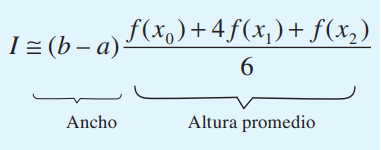
\includegraphics[scale=0.55]{images/trapecio Simpson.png}
            \centering
            \caption{ Fórmula de Simpson $1/3$ representada de la misma forma que el area de un trapecio}
        \end{figure}

        Aplicando la misma secuencia logica vista anteriormente para un polinomio de Lagrange de tercer grado a cuatro puntos obtenemos:
        \begin{equation}
            \begin{split}
                I \cong \frac{3h}{8}[f(x_0) + 3f(x_1) + 3f(x_2) + f(x_3)]
            \end{split}
        \end{equation}

        Donde $h = \frac{(b-a)}{3}$, además de esto a la fórmula anterior se le conoce como \textbf{Regla de Simpson 3/8} debido a que $h$ se multiplica por $\frac{3}{8}$.

    \subsection{Demostraciones de convergencia}
        Dado que Simpson pertenece a la familia de las formulas de integración de Newton-Cotes, podemos ver un patron de convergencia.
        La  Regla del Extremo Izquierdo \cite{openstax_calculusv1} integra exactamente funciones constantes. Tiene una convergencia de $O(h)$. \\
        
        A su vez la Regla del Trapecio integra exactamente funciones lineales. Tiene un convergencia de $O(h^2)$. \\

        El orden n-esimo de la formula de Newton-Cote integra exactamente polinomios hasta el orden $"n"$ converge a $O(h^n+1)$. \\

        Por lo que siendo la Regla de Simpson el segundo orden de la formula de Newton-Cote. Podemos concluir que Simpson converge a $O(h^3)$.

    \subsection{Análisis del error}
    
        Al igual que la regla del trapecio, Simpson $1/3$ se obtiene al integrar el polinomio de interpolacion de Newton-Gregory hacia adelante:
        
        \notag{
            \begin{equation}
                \begin{split}
                    I = \int_{x_0}^{x_2} [f(x_0)+\Delta f(x_0)\alpha + \frac{\Delta ^2 f(x_0)}{2} \alpha (\alpha - 1) \\
                    + \frac{\Delta ^3 f(x_0)}{6} \alpha (\alpha - 1)(\alpha - 2) \\
                    + \frac{f^4(\xi )}{24} \alpha (\alpha - 1)(\alpha - 2) (\alpha - 3)h^4] dx
                \end{split}
            \end{equation}
        }
        
        Vemos que los limites de integracion van de $x_0$ a $x_2$. Por lo tanto, cuando se realizan las sustituciones para simplificar, la
        integral es de $\alpha = 0$ a $2$: 

        \notag{
            \begin{equation}
                \begin{split}
                    I = h \int_0^2 [f(x_0) + \Delta f(x_0) \alpha + \frac{\Delta ^2 f(x_0)}{2} \alpha (\alpha - 1) \\
                    + \frac{\Delta ^3 f(x_0)}{6} \alpha (\alpha - 1)(\alpha - 2) \\
                    + \frac{f^4(\xi )}{24} \alpha (\alpha - 1)(\alpha - 2) (\alpha - 3)h^4] d\alpha
                \end{split}
            \end{equation}
        } \\

        Al integrarse se tiene: 

        \notag{
            \begin{equation}
                \begin{split}
                    I = h[\alpha f(x_0) + \frac{\alpha ^2}{2} \Delta f(x_0) + (\frac{\alpha ^2}{6} - \frac{\alpha ^2}{4}) \Delta ^2 f(x_0) \\
                    + (\frac{\alpha ^4}{24} - \frac{\alpha ^3}{6} + \frac{\alpha ^2}{6}) \Delta ^3 f(x_0) \\
                    + (\frac{\alpha ^5}{120} - \frac{\alpha ^4}{16} + \frac{11 \alpha ^3}{72} - \frac{\alpha ^2}{8}) f^4(\xi) h^4]_0^2
                \end{split}
            \end{equation}
        } \\

        Y evaluando los límites se obtiene: 

        \begin{equation}
            \begin{split}
                I = h[2 f(x_0) + 2 \Delta f(x_0) + \frac{\Delta ^2 f(x_0)}{3} \\
                + (0) \Delta ^3 f(x_0) - \frac{1}{90} f^4(\xi) h^4]
            \end{split}
        \end{equation} \\

        Podemos observar que el coeficiente de la tercera diferencia dividida es cero. Debido a que $\Delta f(x_0) = f(x_1) - f(x_0)$
        y $\Delta ^2 f(x_0) = f(x_2) - 2f(x_1) + f(x_0)$, la ecuación anterior se puede reescribir como: \\
        
        \begin{figure}[H] \label{errorTruncamiento}
            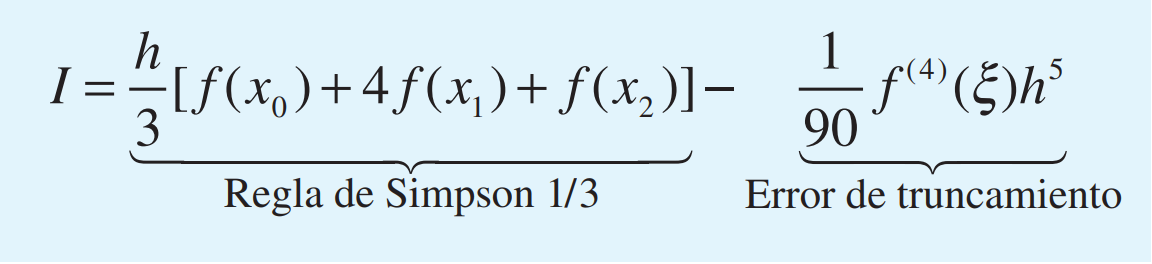
\includegraphics[scale=0.22]{images/error Simpson.png}
            \centering
            \caption{ Fórmula de Simpson $1/3$ junto al error de truncamiento}
        \end{figure}

        Así, el primer término es la regla de Simpson 1/3 y el segundo es el error de truncamiento. Puesto que se suprime la tercera 
        diferencia dividida, se obtiene el resultado significativo de que la fórmula tiene una precisión de tercer orden. \\

        Por otro lado, la regla de Simpson $3/8$ tiene un error de:

        \begin{equation} \tag{33}
            \begin{split}
                E_t = - \frac{3}{80} h^5 f^4(\xi)
            \end{split}
        \end{equation}

        Como podemos observar, en Simpson $3/8$ el denominador es mayor al visto en $1/3$ por lo que podemos decir con seguridad que 
        la Regla de Simpson $3/8$ es más exacta que la Regla de Simpson $1/3$.

    \subsection{Análisis de la eficiencia del método}
        
        Para evidenciar la eficiencia del método se realizara un ejercicio por ambos métodos, obtenido de \cite{chapra_merthod_2007}. \\

        Con la siguiente ecuacion integrar numericamente: $f(x) = 0.2 + 25x -200x^2 +675x^3 -900x^4 +400x^5$ con el intervalo $[0,0.8]$. 
        El valor exacto de la integral es $1.640533$ \\
        
        Haciendo uso de la Regla del Trapecio.
        Al evaluar los limites tenemos:
        \begin{align}
            f(0) &= 0.2 \\
            f(0.8) &= 0.232
        \end{align}

        Sustituyendo:

        \begin{equation} \notag
            I \cong 0.8 \frac{0.2 +  0.232}{2} = 0.1728
        \end{equation}

        La cual representa un error de:

        \begin{equation} \notag
            E_t = 1.640533 - 0.1728 = 1.467733
        \end{equation}

        Ahora utilizando la Regla de Simpson $1/3$:

        Evaluando los limites y el punto medio:
        \begin{align}
            f(0) &= 0.2 \\
            f(0.4) &= 2.456 \\
            f(0.8) &= 0.232
        \end{align} 

        Utilizando figura 1:

        \begin{equation} \notag
            I \cong 0.8 \frac{0.2 + 4(2.456) + 0.232}{6} = 1.367467
        \end{equation}

        Que representa un error exacto de:

        \notag{
            \begin{align}
                E_t &= 1.640533 - 1.367467 = 0.2730667 \\ 
                \varepsilon _t &= 16.6 \% 
            \end{align}
        }

        Que es aproximadamente $5$ veces más precisa que una sola aplicación de la Regla del Trapecio. 
        
    \subsection{Ventajas y desventajas del método}
        \subsubsection{Ventajas}
            \begin{center}
            Ventajas de la Regla de Simpson:
            \end{center}
            \begin{itemize}
                \item   Se obtienen resultados precisos para polinomios cuadraticos y cubicos.
                \item   Es un método con una convergencia más rápida que la regla del trapecio
                \item   La Regla de Simpson $1/3$ alcanza una precision de tercer orden aun cuando se base
                en solo tres puntos, por lo que da resultados exactos para polinomios cubicos aun cuando se obtenga
                de una parabola.
      
            \end{itemize}
        \subsection{Desventajas}
            \begin{center}
            Desventajas de la Regla de Simpson:
            \end{center}
            \begin{itemize}
                \item  La Regla de Simpson $1/3$ es solamente ultilizada cuando el numero de segmentos es par. 
                \item  Por otro lado la Regla de Simpson $3/8$ es utilizada cuando el numero de segmentos es impar. 
                \item  Lo que nos lleva a que en ciertas situaciones sera necesario utilizar tanto la regla $1/3$ como $3/8$
                para obtener un resultado preciso. 
                
            \end{itemize}
    \subsection{Pseudo-código}
        Seudo-código de la Regla de Simpson $1/3$: \\

        $Start$ \\ \\
        $Define$ $Function$ $f(x)$ \\ \\
        $Input$ $lowerLimit, \hspace{0.2cm} upperLimit, \hspace{0.2cm} subInterval$ \\ \\
        $Calculate:$ $stepSize = (lowerLimit - upperLimit)/subInterval$ \\ \\
        $Calculate$ $Integration = f(lowerLimit) + f(upperLimit)$ \\ \\
        $Set:$ $i = 1$ \\ \\
        $Loop$ \\ \\
            $k = lowerLimit + i * stepSize$ \\ \\
            $If (i \hspace{0.2cm} mod \hspace{0.2cm} 3 = 0)$ \\ \\
                $Integration = Integration + 2 * f(k)$ \\ \\
            $Else$ \\ \\
                $Integration = Integration + 4 * f(k)$ \\ \\
            $End$ $If$ \\ \\
            $i = i + 1$ \\ \\
        $While$ $i < = subInterval$ \\ \\
            $Integration = Integration * stepSize/3$ \\ \\
        $Print Integration as Result$ \\ \\
        $Stop$ \\ \\

        Seudo-código de la Regla de Simpson $3/8$: \\

        $Start$ \\
        $Define$ $Function$ $f(x)$ \\ \\
        $Input$ $lowerLimit, \hspace{0.2cm} upperLimit, \hspace{0.2cm} subInterval$ \\ \\
        $Calculate:$ $stepSize = (lowerLimit - upperLimit)/subInterval$ \\ \\
        $Calculate$ $Integration$ $= f(lowerLimit) + f(upperLimit)$ \\ \\
        $Set:$ $i = 1$ \\ \\
        $Loop$ \\ \\
            $k = lowerLimit + i * stepSize$ \\ \\
            $If (i \hspace{0.2cm} mod \hspace{0.2cm} 3 = 0)$ \\ \\
                $Integration = Integration + 2 * f(k)$ \\ \\
            $Else$ \\ \\
                $Integration = Integration + 3 * f(k)$ \\ \\
            $End$ $If$ \\ \\
            $i = i + 1$ \\ \\
        $While$ $i < = subInterval$ \\ \\
        $Integration = Integration * stepSize * 3/8$ \\ \\
        $Print Integration as Result$ \\ \\
        $Stop$ \\ 

    \subsection{Ejemplos}
        Ejemplos del método de Romberg: \cite{chapra_method_2007}
        \subsection{Ejemplo 1}
            Con Simpson $3/8$ integrar en $5$ segmentos: \\

            $f(x) = 0.2 + 25x -200x^2 +675x^3 -900x^4 +400x^5$ con el intervalo $[0,0.8]$ \\

            - Debemos hacer uso de $1/3$ y $3/8$ a la vez. \\

            Los datos necesarios para una aplicación con cinco segmentos $(h = 0.16)$ son:
            \begin{align*}
                f(0) = 0.2         & f(0.16) = 1.296919 \\
                f(0.32) = 1.743393 & f(0.48) = 3.186015 \\
                f(0.64) = 3.181929 & f(0.80) = 0.232
            \end{align*}

            La integral para los dos primeros segmentos se obtiene usando la regla de Simpson $1/3$:

            \begin{equation} \notag
                I \cong 0.32 \frac{0.2 + 4(1.296919) + 1.743393}{6} = 0.3803237
            \end{equation}

            Para los últimos tres segmentos, la regla $3/8$ se utiliza para obtener:

            \begin{equation} \notag
                I \cong 0.48 \frac{1.743393 + 3(3.186015 + 3.181929) + 0.232}{8} = 1.264754
            \end{equation}

            La integral total se calcula sumando los dos resultados:

            \begin{equation} \notag
                I = 0.3803237 + 1.264754 = 1.645077
            \end{equation}

        \subsection{Ejemplo 2}

            Aproxmiar la integral: $\int_1^2 \frac{dx}{x}$ con $n = 2$ subintervalos: \\

            - Hacemos uso de la Regla $1/3$

            \begin{equation} \notag
                I \cong \frac{h}{3}[f(x_0) + 4f(x_1) + f(x_2)]
            \end{equation}

            El ancho del subintervalo es:

            \begin{equation} \notag
                h = \frac{b - a}{n} = \frac{2 - 1}{2} = \frac{1}{2}
            \end{equation}

            Calculando los limites y el valor medio:

            \begin{align*}
                f(x_0) &= 1 \\
                f(x_1) &= \frac{2}{3} \\
                f(x_2) &= \frac{1}{2}
            \end{align*}

            Sustituyendo:

            \begin{equation} \notag
                I \cong \frac{0.5}{3}[1 + 4(\frac{2}{3}) + \frac{1}{2}]
            \end{equation}

            Teniendo finalmente como resultado:

            \begin{equation} \notag
                I = \frac{25}{36} \approx 0.694444 
            \end{equation}

            \section{Cuadratura Gaussiana}
            \subsection{Descripción}
            Gauss plantea tomar puntos de la función que estén ubicados en partes distintas del intervalo para optimizar el cálculo del área o la integral de la manera mas exacta y precisa posible, con Gauss eliminamos la restricción de los puntos fijos sin la necesidad de que estén igualmente espaciados.
            Se plantea de la siguiente manera: 
            
            \begin{figure}[h]
                \centering
                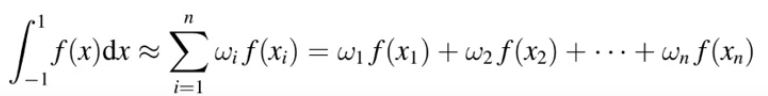
\includegraphics[width=7.5cm ]{images/gauss.PNG}
                \caption{Forma general de la cuadratura de Gauss}
                \label{Formula de Gaussl}
            \end{figure}
            
            
            Consiste en remplazar la integral definida de la función por una sumatoria de coeficientes $c_1$, $c_2$ …$c_n$ multiplicado por los valores evaluados en la función $x_1$, $x_2$ …$x_n$. Entre mas coeficientes de $c$ y $x$ apliquemos, mejor será la precisión y menor será el error de este método. Para obtener los valores para poder realizar el método en dos puntos de integración.
            
            \begin{center}
                $F(x)=1+x+x^2+x^3$
            \end{center}
                
                
            
            
            Debemos utilizar el siguiente polinomio de tercer grado de Gauss que nos garantiza  una integral exacta. 
            
            
            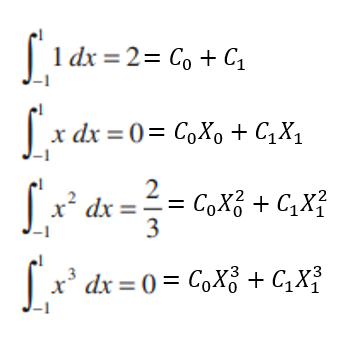
\includegraphics[width=4cm]{images/puntosX_C.PNG}
            
            
            Mediante un sistema de ecuaciones, encontramos las incógnitas faltantes para así poder realizar el método en dos puntos.Así con estos datos podemos encontrar la integral de Gauss para dos puntos, pero realmente podemos utilizar a Gauss para más puntos dependiendo del grado del polinomio y también así aumentando lo máximo posible su precisión.
            
            \begin{align*}
                x_0=\dfrac{1}{\sqrt[]{3}}=0.5773503\\
                x_1=\dfrac{-1}{\sqrt[]{3}}=-0.5773503\\
                c_0=c_1=1
            \end{align*}
             
             Asi, con los polinomios de Legendre podemos obtener tanto los puntos de integracion $x$ y los coeficientes $c$ para $n$ puntos distintos, en la siguiente tabla se muestran los valores hasta para 5 puntos:
             
                \begin{table}[h]
                    \begin{center}
                        \caption{Valores de $x$ y $c$ hasta 5 puntos}
                        \begin{tabular}{| c | c | c | c |}
                            \hline
                        Puntos & Pesos & Valores de la funcion \\ \hline
                         2& $c_0$ = 1 & $x_0$ = –0.577350269   \\
                         & $c_1$ = 1 &$x_1$ = 0.577350269   \\ \hline
                        & $c_0$ = 0.5555556 & $x_0$ = –0.774596669  \\ 
                         3& $c_1$ = 0.8888889 & $x_1$ = 0  \\ 
                         & $c_2$ = 0.5555556  & $x_2$ = 0.774596669  \\ \hline
                         & $c_0$ = 0.3478548 & $x_0$ = –0.861136312  \\ 
                         4& $c_1$ =  0.6521452 & $x_1$ =  –0.339981044  \\ 
                         & $c_2$ =  0.6521452 & $x_2$ =  0.339981044  \\ 
                         & $c_3$ = 0.3478548  & $x_3$ = 0.861136312 \\ \hline
                         & $c_0$ = 0.2369269 & $x_0$ = –0.906179846   \\ 
                         & $c_1$ = 0.4786287  & $x_1$ = –0.538469310  \\ 
                         5& $c_2$ =  0.5688889 & $x_2$ = 0  \\ 
                         & $c_3$ = 0.4786287 & $x_3$ = 0.538469310  \\ 
                         & $c_4$ = 0.2369269  & $x_4$ = 0.906179846 \\ \hline
                         
                        \end{tabular}
                        \label{tab:ejemploTablaGauss}
                    \end{center}
                        \end{table}
             
             Los limites de integracion fueron especificados de -1 a 1 para poder hacer el metodo mas simple y general posible, pero la mayoria de las funciones no cumpliran estos limites, es por eso que se necesita realizar una transformacion de los intervalos de integracion.
            
            \begin{figure}[h]
                \centering
                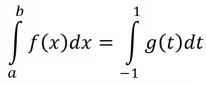
\includegraphics[width=3cm]{images/transformacionlimites.PNG}
            \end{figure}
            Siendo $a$ nuestro limite inferior y $b$ nuestro limite superior podemos hacer lo siguiente:
            
            \begin{align*}
               x=\dfrac{(b+a)+(b-a)x_d}{2},dx=\dfrac{(b-a)}{2}dx_d
            \end{align*}
            una vez tenemos $x$ y $dx$ podemos remplazarla en nuestra integral original, y asi obtener nuestra nueva funcion $g(x)$ transformada a sus nuevos limites de -1 a 1.
            
            
            \subsection{Demostraciones de convergencia}
            Las aplicaciones de la cuadratura Gaussiana son de una gran sustento matematico para las integrales, el calculo de areas bajo la curva e interpolacion de polinomios, Dada su naturaleza creciente de valores de n, esto hace que su aceleracion de convergencia sea mayor conforme mas nodos o mas grados tenga el polinomio, en el siguiente grafico se muestra la convergencia, en función del grado n de Legendre:
            
            \begin{figure}[h]
                \centering
                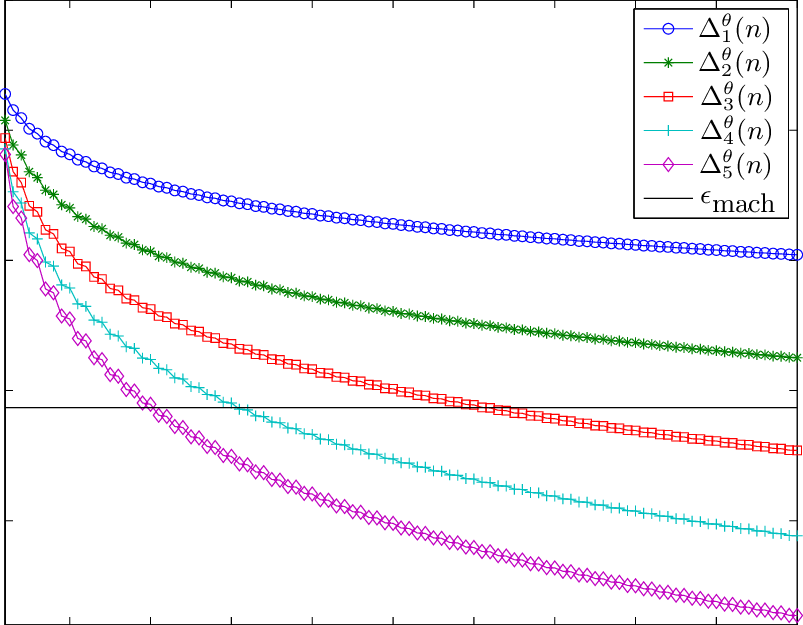
\includegraphics[width=\linewidth]{images/Convergencia_Gauss.png}
                \caption{Convergencia de Gauss - Legendre}
                \label{fig:función del grado n de Legendre}
            \end{figure}
            
            Esto implica una complejidad O(n) para n puntos, donde los polinomios de lagrenge van obteniendo una mayor precision mientras aumentan los nodos.
            
            \begin{align*}
                I_1 = c_0f(x_0)+c_1f(x_1)\\
                I_2= c_0f(x_0)+c_1f(x_1)+c_2f(x_2)\\
                .\\
                .\\
                .\\
                I_n= c_0f(x_0)+c_1f(x_1)+c_2f(x_2)+c_n+f(x_n)
            \end{align*}
            
            
            \subsection{Análisis del error}
            Para el analisis del error necesitamos una tolerancia que este alojada entre los limites arbitrarios desde -1 a 1 donde n es el numero de nodos menos 1, aunque sea la formula de integracion de Gauss mas utilizada, este metodo presenta un error mas grande o pequeño dependiendo sobre todo del numero de nodos que se use, la formula para el analisis del error es la siguiente: 
            
            \begin{figure}[h]
                \centering
                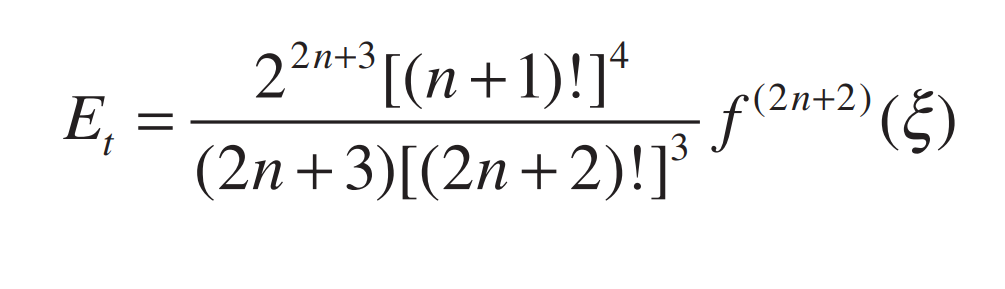
\includegraphics[width=\linewidth]{images/error_gauss.PNG}
                \caption{Formula del error de Cuadratura Gaussiana}
                \label{fig:Formula_error_Gauss}
            \end{figure}
            
            
            
            
            \subsection{Análisis de la eficiencia del método}
            Las diferentes aplicaciones de Cuadratura suelen necesitar un numero pequeño de nodos para funcionar pero muchas veces la cuadratica gaussiana necesita mas nodos de lo habitual haciendo otros metodos de cuadratura mas calificados.
            
            \vspace{2mm}
            
            a continuacion las tabla con los distintos tipos de errores que presentan los distintos metodos de cuadratura y su efeciencia en nodos y pesos: 
            
            \vspace{2.6cm}
            
            \begin{figure}[h]
                \centering
                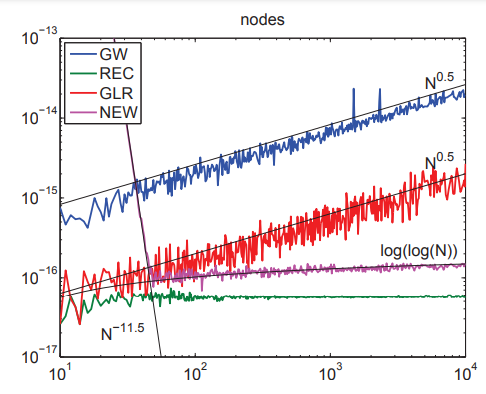
\includegraphics[width=\linewidth]{images/eficiencia_metodos_nodos.PNG}
                \caption{Grafica comparativa de eficiencia en los nodos}
                \label{fig:Eficiencia en los nodos}
            \end{figure}
            
            \begin{figure}[h]
                \centering
                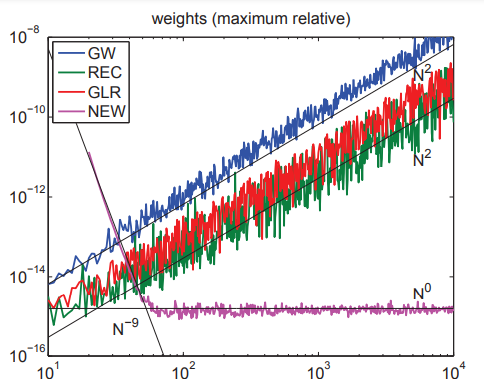
\includegraphics[width=\linewidth]{images/eficiencia_metodos_pesos.PNG}
                \caption{Grafica comparativa de eficiencia en los pesos}
                \label{fig:Eficiencia en los pesos}
            \end{figure}
            
            Como se puede ver en las tablas, la complejidad y eficiencia de la cuadratura Gaussiana empeora conforme $n$ va en aumento, mientras que nuevos metodos basados en el metodo de newton son muy efectivos en los casos donde la $n$ es un numero bastante mas grande.
                        
                            \begin{table}[h]
                    \begin{center}
                        \caption{Tabla comparativa de error y rapidez}
                        \begin{tabular}{| c | c | c | c |}
                            \hline
                        Metodo & $E_{abs}$ $\lbrace$$x_k$$\rbrace$ & $E_{rm}$ $\lbrace$$w_k$$\rbrace$ &Rapidez\\ \hline 
                        GW & $O(\sqrt{n})$ & $O(n^{3/2})$ & $O(n^2)$ \\
                        REC & $O(1)$ & $O(n)$ & $O(n^{1.7})$ \\
                        GLR & $O(\sqrt{n})$ & $O(n)$ & $O(n)$ \\
                        NEW & O($log$($log$(n))) & O($log$($log$(n))) & $O(n)$ \\ \hline
                        \end{tabular}
                        \label{tab:tabla de error y rapidez}
                    \end{center}
                        \end{table}
            
            
            \subsection{Ventajas y desventajas del método}
                \subsubsection{Ventajas}
                        \begin{itemize}
                            \item   Es una de los metodos mas rapidos de todos a pesar de tener que aumentar su numero de nodos y evaluaciones. 
                            \item   No necesita puntos de evaluacion que este igualmente separados entre si ya que los selecciona de la manera mas optima.
                            \item tanto los pesos como los valores de evaluacion ya estan arbitrareamente dados, solo dependera de cuantos nodos tiene o el grado del polinomio
            
                    \end{itemize}
                \subsubsection{Desventajas}
                        \begin{itemize}
                            \item  Entre mas rigurosa sea la tolerancia habra que aumentar el numero de nodos teniendo asi que hacer mas evaluaciones.
                            \item   Al estar limitada solo entre los intervalos [-1,1], puede que algunas funciones presenten singularidades
                            \item   Los puntos de evaluacion van cambiando conforme con los anteriores
                            
            
                    \end{itemize}
                
            \subsection{Pseudo-código}
                    Seudo-código del la Cuadratura Gaussiana: \cite{in_mr} \\
            
                    ENTRADA: Limites de integracion a, b, F funcion a evaluar y m numero de nodos \\
                    SALIDA: Integral calculada 
                    (se guardan en almacenamiento) \\
                    PROCESO: \\
                    
                            \begin{itemize}
                        \item   PASO 1; Se opera $c_1=(b+a)/2$ y $c_1=(b-a)/2$. \\
                        \item   PASO 2; El FOR desarrollla la sumatoria y evalua en la funcion a partir de los valores anteriores.\\
                        \item   PASO 3; Por ultimo se calcula la integral sustituyendo el resultado de la sumatoria en la ecuacion general de la cuadratura Gaussiana.\\
                        \item   PASO 4; se imprime el resultado. \\
                    \end{itemize}
                    
                            Pseudo-código más detallado: \cite{Numerical Methods in Engineering with Python 3} \\
                    $FUNCTION$ $ gaussQuad (f,a, b, m,)$ \\
                    $c_1=(b+a)/2$ \\
                    $c_2=(b-a)/2$ \\
                    $x,A = gaussNodes(m)$ \\
                    $sum = 0.0$\\
                    $DO FOR$ $K=X$\\
                    $ITER = ITER +1 $\\
                    $sum = sum + A[ITER]*f(c1 + c2*x[ITER])$\\
                    $END DO$\\
                    $return$ $ c2*sum$\\
                    $END$ $gaussQuad$ 
            
            \subsection{Ejemplos}
            Aplicaremos la cuadratura gaussiana para encontrar el area  bajo la curva de la siguiente integral:
            
            
                \begin{equation} 
                    \int_0^3 f(x)=\frac{e^xsen(x)}{1+x^2} dx
                \end{equation}
                
                \begin{enumerate}
                    \item Primero necesitaremos hacer el cambio de limites de [0,3] a [-1,1] a traves de las formulas ya vistas:
                    
                    \begin{align*}
                        x=\dfrac{(b+a)+(b-a)x_d}{2},dx=\dfrac{(b-a)}{2}dx_d
                    \end{align*}
                    
                    \item Evaluamos las variables [0,3] en a y b:
                    
                     \begin{equation*}
                        x=\dfrac{(3+0)+(3-0)x}{2}=\dfrac{3}{2}x+\dfrac{3}{2}
                    \end{equation*}
                    
                    \begin{equation*}
                        dx=\dfrac{(3-0)}{2}dx=\dfrac{3}{2}dx
                    \end{equation*}
                    
                    \item Ahora remplazamos $x$ y $dx$ en nuestra funcion:
                    
                    \begin{equation*} 
                        f(\frac{3}{2}x_n+\frac{3}{2})=\frac{e^{\frac{3}{2}x_n+\frac{3}{2}}sen(\frac{3}{2}x_n+\frac{3}{2})}{1+(\frac{3}{2}x_n+\frac{3}{2})^2} 
                    \end{equation*}
                    
                    \item Evaluamos $x_n$ con los coeficientes de la cuadratura gaussiana para 2 puntos: 
                    
                    
                    \begin{multline*}
                        f(\frac{3}{2}x_0+\frac{3}{2})=\\
                        \\
                        \frac{e^{\frac{3}{2}(-0.5773502)+\frac{3}{2}}sen(\frac{3}{2}(-0.5773502)+\frac{3}{2})}{1+(\frac{3}{2}(-0.5773502)+\frac{3}{2})^2} \\
                        =0.796501031
                    \end{multline*}
                    
                            \begin{multline*}
                        f(\frac{3}{2}x_1+\frac{3}{2})=\\
                        \\
                        \frac{e^{\frac{3}{2}(0.5773502)+\frac{3}{2}}sen(\frac{3}{2}(0.5773502)+\frac{3}{2})}{1+(\frac{3}{2}(0.5773502)+\frac{3}{2})^2}\\
                        =1.130596636
                    \end{multline*}
                    
                    \item Una vez contamos con todos los datos solo debemos realizar la sumatoria:
                    
                    \begin{equation*}
                        I=\frac{3}{2}[w_0f(\frac{3}{2}x_0+\frac{3}{2})+w_1f(\frac{3}{2}x_1+\frac{3}{2})]
                    \end{equation*}
                    
                    \begin{equation*}
                        I=\frac{3}{2}[(1)(0.796501031)+(1)(1.130596636)]
                    \end{equation*}
                    
                    \item Dandonos como respuesta final:
                    
                            
                    \begin{equation*}
                        I=2.890646501
                    \end{equation*}
                    
                \end{enumerate}
                
                En este caso tenemos un error algo elevado ya que el valor teorico de la integral es de $2.88163$, por lo que si quisieramos obtener una valor mas exacto deberiamos aumentar el numero de nodos.
            
\section{Diferencia Media}
\subsection{Descripción}
\begin{lipsum}
    Teorema de Diferencia Media
\end{lipsum}
\subsection{Demostraciones de convergencia}
\begin{lipsum}
    Demostraciones de convergencia
\end{lipsum}
\subsection{Análisis del error}
\begin{lipsum}
    Análisis del error
\end{lipsum}
\subsection{Análisis de la eficiencia del método}
\begin{lipsum}
    Análisis de la eficiencia del método
\end{lipsum}
\subsection{Ventajas y desventajas del método}
\begin{lipsum}
    Ventajas y desventajas del método
\end{lipsum}
\subsection{Pseudo-código}
\begin{lipsum}
    Pseudo-código
\end{lipsum}
\subsection{Ejemplos}
\begin{lipsum}
    An article \cite{anarticle}
\end{lipsum}
\newpage
\section{Bibliografía}
\bibliographystyle{IEEEtran}
\bibliography{Proyecto}
\end{document}

